%
% simrecomb_docs.tex
%
% Copyright 2012 Darren Kessner
%
%   Licensed under the Apache License, Version 2.0 (the "License");
%   you may not use this file except in compliance with the License.
%   You may obtain a copy of the License at
%
%       http:%www.apache.org/licenses/LICENSE-2.0
%
%   Unless required by applicable law or agreed to in writing, software
%   distributed under the License is distributed on an "AS IS" BASIS,
%   WITHOUT WARRANTIES OR CONDITIONS OF ANY KIND, either express or implied.
%   See the License for the specific language governing permissions and
%   limitations under the License.
%

\documentclass{article}

\usepackage{graphicx}

% for 8.5 x 11 with pdflatex
\pdfpagewidth=\paperwidth 
\pdfpageheight=\paperheight


\begin{document}

\title{\texttt{simrecomb}}
\author{Darren Kessner}
\maketitle

%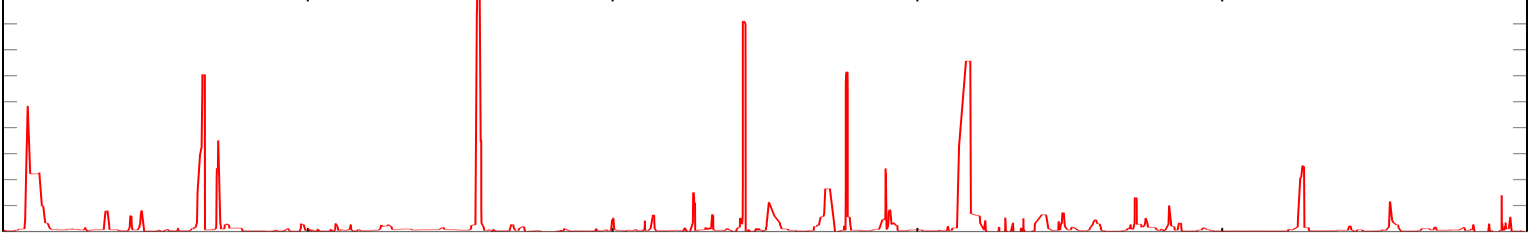
\includegraphics[width=1.0\textwidth]{fig/hotspots_bare.png}


\section{Introduction}


\texttt{simrecomb} is a command-line program for simulating recombination and
admixture among multiple populations over multiple non-overlapping generations.
The user can specify population sizes, admixture rules for each population in
each generation, and genetic maps for recombination rates along chromosomes.
Individuals are diploid, and can have multiple chromosomes.  Individual
chromosome blocks are tracked during the course of the simulation, with
identifiers specifying the exact ancestral individual from which the block is
derived.

\begin{center}
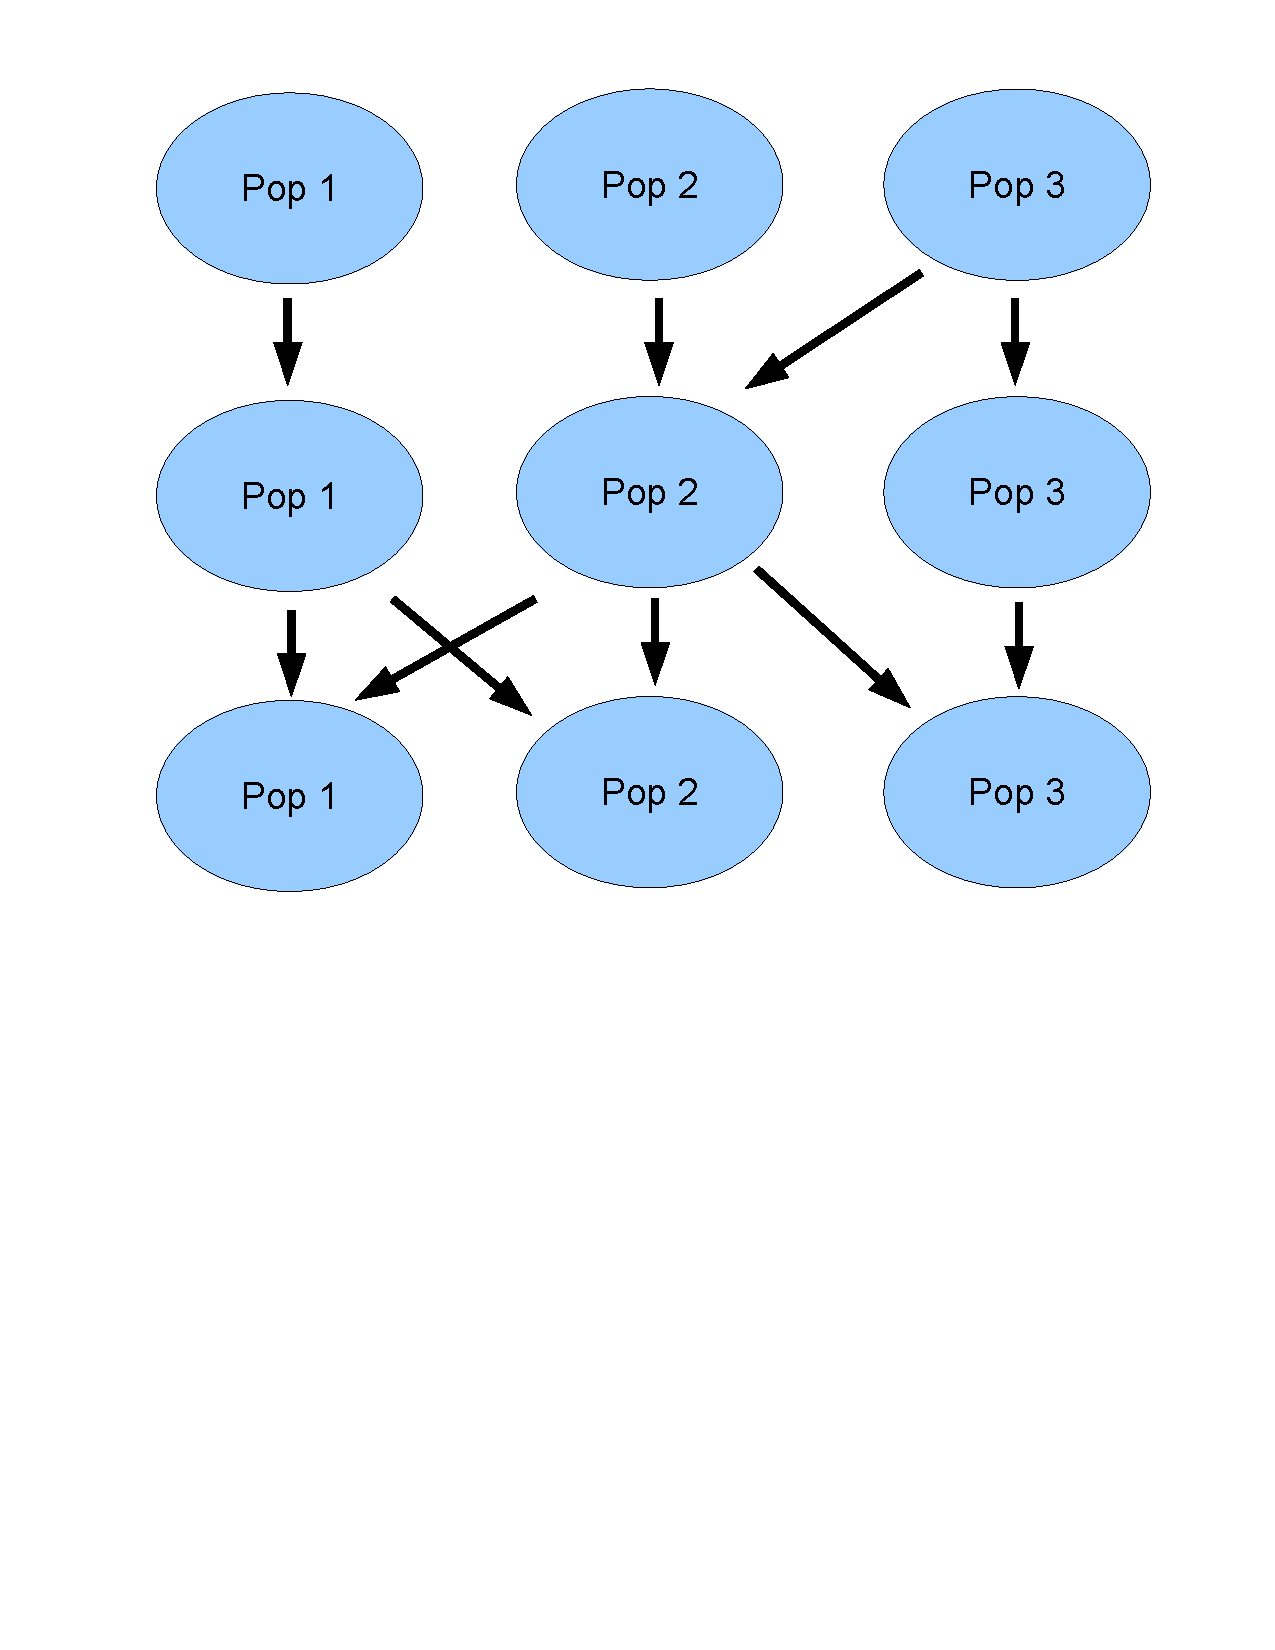
\includegraphics[width=.50\textwidth]{fig/simrecomb_cartoon.pdf}
\end{center}



\section{Usage}



\end{document}


